\documentclass[fleqn,compress,utf8,aspectratio=169,t]{beamer}
% use LMU theme
\usetheme{LMU}

% This setups a lot of recommended settings and packages you usually need
% anyway. So let me take care for you and your document stays clear.

% Examples: Tables, Graphics, Listings, Hyperref...
%
% Prevent slide breaks in the middle of a paragraph
\widowpenalties 1 10000
\raggedbottom

\makeatletter
\@ifundefined{KOMAClassName}{% if non-KOMA class
  \IfFileExists{parskip.sty}{%
    \RequirePackage{parskip}
  }{% else
    \setlength{\parindent}{0pt}
    \setlength{\parskip}{6pt plus 2pt minus 1pt}}
}{% if KOMA class
  \KOMAoptions{parskip=half}}
\makeatother

\IfFileExists{xurl.sty}{\usepackage{xurl}}{} % add URL line breaks if available
\IfFileExists{bookmark.sty}{\usepackage{bookmark}}{\usepackage{hyperref}}
\urlstyle{same} % disable monospaced font for URLs

\usepackage{listings}
\lstset{defaultdialect=[5.3]Lua}
\lstset{defaultdialect=[x86masm]Assembler}
\usepackage{longtable,booktabs}
\usepackage{caption}
% Make caption package work with longtable
\makeatletter
\def\fnum@table{\tablename~\thetable}
\makeatother
\usepackage{graphicx}
\makeatletter
\def\maxwidth{\ifdim\Gin@nat@width>\linewidth\linewidth\else\Gin@nat@width\fi}
\def\maxheight{\ifdim\Gin@nat@height>\textheight\textheight\else\Gin@nat@height\fi}
\makeatother
% Scale images if necessary, so that they will not overflow the page
% margins by default, and it is still possible to overwrite the defaults
% using explicit options in \includegraphics[width, height, ...]{}
\setkeys{Gin}{width=\maxwidth,height=\maxheight,keepaspectratio}
% Set default figure placement to htbp
\makeatletter
\def\fps@figure{htbp}
\makeatother
\usepackage[normalem]{ulem}
% Avoid problems with \sout in headers with hyperref
\pdfstringdefDisableCommands{\renewcommand{\sout}{}}
\setlength{\emergencystretch}{3em} % prevent overfull lines
%Tightlist Command
\providecommand{\tightlist}{%
  \setlength{\itemsep}{0pt}\setlength{\parskip}{0pt}}



\usepackage[style=ieee]{biblatex}
\addbibresource{slides.bib}
\usepackage{tikz}
\usepackage{amsmath}
\usepackage[utf8]{inputenc}
\usepackage{pgf-umlsd}
\usetikzlibrary{timeline}
\usetikzlibrary{decorations.pathreplacing}

%%%%%%%%%%%%%%%%%%%%%%%%%%%%%%%%%%%%%%%%%%%%%%%%%%%%%%%%%%%%%%%%%%%%%%%%%%%%%%%%
%%                                 Customizations                             %%
%%%%%%%%%%%%%%%%%%%%%%%%%%%%%%%%%%%%%%%%%%%%%%%%%%%%%%%%%%%%%%%%%%%%%%%%%%%%%%%%

% If you want no navigation uncomment this
%\beamertemplatenavigationsymbolsempty

% setup listings
\lstset{
  basicstyle=\ttfamily\color{black},
  showstringspaces=false
}

\lstdefinestyle{highlight}{
  keywordstyle=\color{red},
  commentstyle=\color{lmu@darkgray}
}

\lstdefinestyle{basetex}{
language={[LaTeX]Tex}, 
basicstyle=\color{black!40},
keywordstyle=\color{red!40},
commentstyle=\color{lmu@darkgray!40},
moredelim=**[il][\only<+>{\color{black}\lstset{style=highlight}}]{@}
}

\lstdefinestyle{basec}{
language=C,
basicstyle=\color{black!40},
keywordstyle=\color{red!40},
commentstyle=\color{green!40},
moredelim=**[il][\only<+>{\color{black}\lstset{style=highlight}}]{@}
}

%%%%%%%%%%%%%%%%%%%%%%%%%%%%%%%%%%%%%%%%%%%%%%%%%%%%%%%%%%%%%%%%%%%%%%%%%%%%%%%%
%%                                  Title Page Data                           %%
%%%%%%%%%%%%%%%%%%%%%%%%%%%%%%%%%%%%%%%%%%%%%%%%%%%%%%%%%%%%%%%%%
% helper command to add multiple authors
\newcommand{\newauthor}[2]{
\parbox[c]{0.26\textwidth}{
{\bfseries #1} \\
{\scriptsize{\href{mailto:#2}{#2}}}
}
%{#1}
}

% Authors
\author[Lösch]{
  \newauthor{Robin Lösch}{loesch@cip.ifi.lmu.de} 
}

\date[\today]{\today}

\title{Quantum Secure Key Exchange for IEEE 802.1AE (MACSec)}
\subtitle{Antrittsvortrag zur Masterarbeit}

\hypersetup{
  pdftitle={Title},
  pdfauthor={Author},
  hidelinks}


%%%%%%%%%%%%%%%%%%%%%%%%%%%%%%%%%%%%%%%%%%%%%%%%%%%%%%%%%%%%%%%%%%%%%%%%%%%%%%%%
%%                                  Document                                  %%
%%%%%%%%%%%%%%%%%%%%%%%%%%%%%%%%%%%%%%%%%%%%%%%%%%%%%%%%%%%%%%%%%%%%%%%%%%%%%%%%

\begin{document}

\begin{frame}
  \titlepage
\end{frame}

%%%%%%%%%%%%%%%%%%%%%%%%%%%%%%%%%%% Overview %%%%%%%%%%%%%%%%%%%%%%%%%%%%%%%%%%%

\section{Overview}

\subsection{Motivation}


\section{Media Access Control Security}

\begin{frame}{IEEE 802.1X}
  \begin{columns}[t]
    \column{.4\textwidth}
  \begin{itemize}
    \item Mutual authentication in LANs
    \begin{itemize}
      \item<2-> Supplicant (Peer)
      \item<3-> Authenticator (Switch)
      \item<4-> Radius (AAA Server)
    \end{itemize}
    \item<5-> Mutually trusted CAs (c)
    \item<6-> EAP framework (e,f)
    \begin{itemize}
      \item Asymmetric key exchange
    \end{itemize}
  \end{itemize}
    \column{.6\textwidth}
      \begin{figure}[t]
        \centering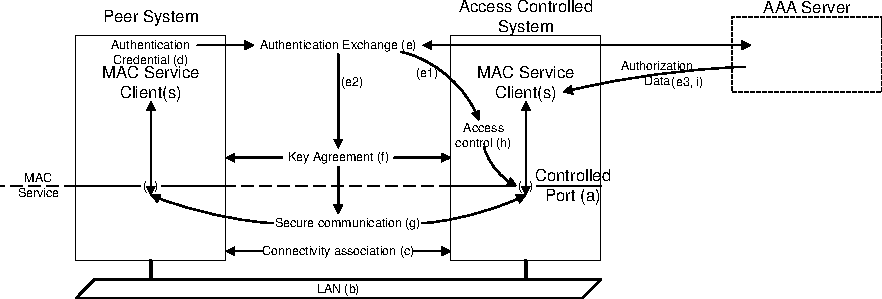
\includegraphics[trim={0 0 0 0}, clip, width=1.0\columnwidth]{8021x_fig_6_1_overview.pdf}
    \end{figure}
    
  \end{columns}
  
\end{frame}

\begin{frame}{IEEE 802.1AE (MACSec)}
  \begin{columns}[t]
    \column{.5\textwidth}
    \begin{itemize}
      \item Ethernet frame encryption
      \begin{itemize}
        \item<2-> Uses 802.1X CAs for authentication
        \item<3-> Uses MKA for symmetric key exchange
      \end{itemize}
    \end{itemize}
    \column{.5\textwidth}
    \vspace*{-1cm}
      \begin{figure}[t]
        \centering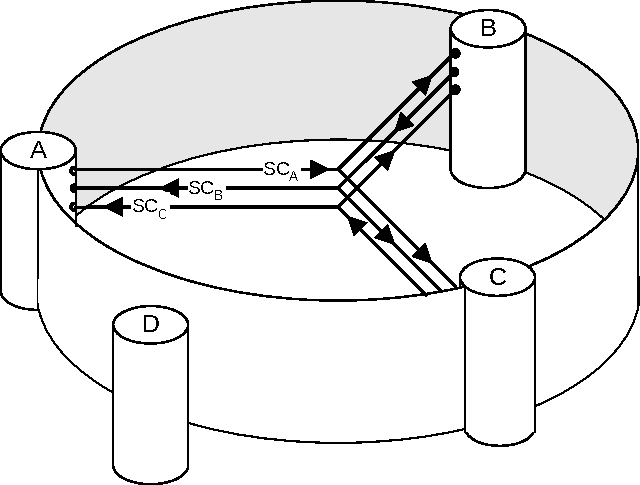
\includegraphics[trim={0 0 0 2}, width=1\columnwidth]{8021ae_fig_7_6_ca.pdf}
    \end{figure}
    
  \end{columns}
\end{frame}


\begin{frame}{Motivation}
  \begin{itemize}
    \item Quantum Computing is a ``Hype Topic''
    \item<2-> Faster algorithms:
          \begin{itemize}
            \item Search problems
            \item Optimizations (Adiabatic QC)
          \end{itemize}
     \item<3-> New algorithms:
          \begin{itemize}
            \item Quantum teleportation
          \end{itemize}
  \end{itemize}
\end{frame}

\begin{frame}{Motivation}
  \begin{itemize}
  \item Efficient solution for (some) computational problems
  \item <2-> Modern crypto is based in such problems:
  \begin{itemize}
    \item<3-> Grover's search algorithm \\
      \onslide<4->Reduce symmetric crypto keyspace by \(\mathcal{O}(\sqrt{n})\)
    \item<5-> Shor's factorization algorithm \\
      \onslide<6-> Breaks (EC)DH and RSA based crypto in polynomial time
  \end{itemize}
\end{itemize}
\end{frame}

\begin{frame}{Practical Quantum Computer}
  \begin{columns}[t]
    \column{.4\textwidth}
    When to panic?
    \begin{itemize}
    \item<2-> \#Qubits to break a n-bit key
    \begin{itemize}
      \item RSA:  \(2n+2\) \cite{haner2016factoring}
      \item DLP:  \(9n+2\ln(n)\) \cite{roetteler2017quantum}
    \end{itemize}
    \item<3-> Coherency time
    \begin{itemize}
      \item Keeping a state is tricky
      \item Implementation dependent
      \item Hard to predict
    \end{itemize}
  \end{itemize}
  \column{.6\textwidth}
    \vspace*{-1cm}
      \begin{figure}[t]
        \centering\includegraphics<2->[trim={10px 0 0 10px}, clip, width=1\columnwidth]{plot_line_shor_rsa.pdf}
    \end{figure}
  \end{columns}
\end{frame}

\begin{frame}{Practical Quantum Computer}
  \begin{itemize}
  \item<1-> Even if we assume a Moore-like exp growth we still got plenty of time
  \item<2-> We should use this time!
  \begin{enumerate}
    \item<3-> {Design quantum safe algorithms}
    \item<4-> \textbf{Implement quantum safe algorithms}
  \end{enumerate}
\end{itemize}
\end{frame}


\section{Developing New Algorithms}

\begin{frame}{NIST PQ Project}
  \begin{itemize}
  \item<1-> Start Dec 20, 2016
  \item<1-> 3. Round announced Jul 22, 2020
  \item<2-> Goal: Select quantum safe key exchange and signature algorithms
\end{itemize}
\end{frame}

\begin{frame}{A clear winner?}
  \begin{columns}[t]
    \column{.4\textwidth}
    \begin{itemize}
      \item<2-> Different Foundations
      \begin{itemize}
        \item Lattice-based
        \item Isogeny-based
        \item Code-based
      \end{itemize}
    \end{itemize}
    \bigskip
    \begin{itemize}
      \item<3-> Different Trade-offs
      \begin{itemize}
        \item Latency
        \item Key size
        \item Maturity
      \end{itemize}
    \end{itemize}

    \column{.6\textwidth}
    \vspace*{-1cm}
      \begin{figure}[t]
        \centering\includegraphics<3->[trim={20px 0 0 40px}, clip, width=1\columnwidth]{plot_scatter_all_latency_pubkeysize.pdf}
    \end{figure}
    
  \end{columns}
\end{frame}


\section{Implementing New Algorithms}

\begin{frame}{Requirements on Public Key Crypto}
  \begin{itemize}
    \item Web-Server
    \begin{itemize}
      \item Thousands of handshakes/s
      \item Forward secrecy
    \end{itemize}
  \end{itemize}
  \pause
  \begin{itemize}
    \item IoT \& WSN
    \begin{itemize}
      \item Small traffic volume
    \end{itemize}
  \end{itemize}
  \pause
  \begin{itemize}
    \item Long-term signatures
    \begin{itemize}
      \item Maturity
    \end{itemize}
  \end{itemize}
\end{frame}

\begin{frame}{Existing Applications}
  \begin{itemize}
    \item Internet-Drafts for TLS 1.X\cite{ietf-tls-hybrid-design-00}\cite{whyte-qsh-tls13-06}\cite{schanck-tls-additional-keyshare-00}\cite{kiefer-tls-ecdhe-sidh-00}\cite{whyte-qsh-tls12-02}
    \item QuaSiModO: Quantum resistant IKEv2\cite{exchangetowards}
    \item ``New Hope'' in Google Chrome\cite{cecpq1}
  \end{itemize}
\end{frame}

\section{Outline}

\begin{frame}{Why 802.1(X|AE)?}
  \begin{itemize}
    \item Widely used in practice
    \begin{itemize}
      \item<2-> Enterprise LANs
      \item<2-> WPA2-Enterprise
    \end{itemize}
    \item<3-> Heterogeneous environments
    \begin{itemize}
      \item<4-> Data centers \(\Leftrightarrow\) IoT networks
      \item<4-> Helps understanding algorithms 
    \end{itemize}
    \item<5-> Industry relevance
    \begin{itemize}
      \item<6-> Part of QuaSiModO/ADVA cooperation
    \end{itemize}
  \end{itemize}

\end{frame}


\begin{frame}{Goals}
  \begin{itemize}
    \item<2->  Evaluation of IEEE 802.1(X|AE)
    \begin{itemize}
      \item<3->  Identify vulnerable components
      \item<3->  Extract requirements for quantum safe design
    \end{itemize}
    \item<4-> Evaluation of quantum safe algorithms
    \item<5-> Design of a quantum safe alternative
    \item<6-> Implementation in a real-world test-case
    \item<7-> Extensive experimental evaluation
  \end{itemize}
\end{frame}

\begin{frame}{}
  \hspace*{-1.81cm}
    \begin{tikzpicture}[timespan={},timeline width=16]
      \timeline[custom interval=true]{\bfseries \small Week 0, \bfseries   \small Week 4, \small  \bfseries Week 8,  \small \bfseries Week 12,  \small \bfseries Week 16,  \small \bfseries Week 20,  \small \bfseries Week 24}
      \begin{phases}
        \initialphase{involvement degree=1.75cm,phase color=black,phase opacity=0}
        \phase{between week=1 and 2 in 0.5,involvement degree=3.25cm,phase color=blue!80!cyan}
        \phase{between week=3 and 4 in -0.1,involvement degree=2.7cm,phase color=green!50!black}
        \phase{between week=4 and 5 in 0,involvement degree=2.25cm,phase color=orange!50!black}
        \phase{between week=5 and 6 in 0.3,involvement degree=4.25cm,phase color=red!50!black}
        \phase{between week=6 and 7 in 0.8,involvement degree=3cm,phase color=black}
      \end{phases}
      \onslide<2>\addmilestone{at=phase-1.90,direction=90:1.2cm,text={\textbf{Background \& Related Work}},text options={above}}
      \onslide<3->\addmilestone{at=phase-1.90,direction=90:1.2cm,text={Background \& Related Work},text options={above}}
      \onslide<3>\addmilestone{at=phase-2.270,direction=270:0.8cm,text={\textbf{Requirement Analysis}},text options={below}}
      \onslide<4->\addmilestone{at=phase-2.270,direction=270:0.8cm,text={Requirement Analysis},text options={below}}
      \onslide<4>\addmilestone{at=phase-3.90,direction=90:0.8cm,text={\textbf{Design}},text options={above}}
      \onslide<5->\addmilestone{at=phase-3.90,direction=90:0.8cm,text={Design},text options={above}}
      \onslide<5>\addmilestone{at=phase-4.110,direction=120:1.5cm,text={\textbf{Implementation}},text options={above}}
      \onslide<6->\addmilestone{at=phase-4.110,direction=120:1.5cm,text={Implementation},text options={above}}
      \onslide<6>\addmilestone{at=phase-5.270,direction=270:0.5cm,text={\textbf{Evaluation}},text options={below}}
      \onslide<7->\addmilestone{at=phase-5.270,direction=270:0.5cm,text={Evaluation},text options={below}}
      \onslide<7>\addmilestone{at=phase-5.40,direction=70:0.5cm,text={\textbf{Finalization}},text options={above}}
      \onslide<8->\addmilestone{at=phase-5.40,direction=70:0.5cm,text={Finalization},text options={above}}
      \draw<8-> [decorate,decoration={brace,mirror,amplitude=10pt},xshift=-4pt,yshift=0pt]
  (1.6,0) -- (9.1,0)node [midway,xshift=0pt,yshift=-22pt] {\small\textbf{Paperwork}};
  \draw<8-> [decorate,decoration={brace,mirror,amplitude=10pt},xshift=-4pt,yshift=0pt]
  (12.33,0) -- (15.15,0)node [midway,xshift=0pt,yshift=-22pt] {\small\textbf{Paperwork}};
      \onslide<1->  
    \end{tikzpicture}
\end{frame}

\begin{frame}

    \begin{center}
    \tikzset{
      % add this style to all tikzpicture environments
      every picture/.append style={
        % enable scaling of nodes
        transform shape,
        % set scale factor
        scale=0.6
      }
    }
  \begin{sequencediagram}
    \renewcommand\unitfactor{0.5}
    \newthread[white]{c}{Client}
    \newinst[4]{a}{Authenticator}
    \newinst[4]{s}{Auth. Server}

    \onslide<2->\mess[1]{c}{EAPOL|EAP|TLS}{a}
    \onslide<3->\mess[1]{a}{RADIUS|EAP|TLS}{s}
    \onslide<3->\mess[1]{s}{RADIUS|EAP|TLS}{a}
    \onslide<4->\mess[1]{a}{RADIUS}{s}
    \onslide<4->\mess[1]{s}{RADIUS}{a}
    \onslide<5->\mess[1]{a}{EAPOL|EAP}{c}
    \onslide<6->\mess[1]{c}{EAPOL|MKA}{a}
    \onslide<6->\mess[1]{a}{EAPOL|MKA}{c}
    \onslide<7->\mess[1]{c}{MACSec|*}{a}

\end{sequencediagram}
\end{center}

\end{frame}


\begin{frame}{A short history of quantum computing}
  \begin{columns}[t]
    \hspace*{-4.7cm}
    \column{1\textwidth}
    \vspace*{-1cm}
    \begin{figure}
      \begin{tikzpicture}[timeline width=16,timespan={}]
        \timeline[custom interval=true]{\bfseries 1980, \bfseries \dots,\bfseries 1996, \bfseries 1999, \bfseries 2001, \bfseries \dots, \bfseries 2019, \bfseries \dots, \bfseries 2030}
        \begin{phases}
          \initialphase{involvement degree=1.75cm,phase color=black, phase opacity=0}
            \phase{between week=1 and 2 in 0,involvement degree=2.25cm}
            \phase{between week=3 and 4 in 0,involvement degree=2.25cm,phase color=blue!80!cyan}
            \phase{between week=4 and 5 in 0,involvement degree=2.25cm,phase color=green!50!black}
            \phase{between week=5 and 6 in 0,involvement degree=2.25cm,phase color=orange!50!black}
            \phase{between week=7 and 8 in 0,involvement degree=2.25cm,phase color=red!50!black}
            \phase{between week=8 and 9 in 1,involvement degree=2.25cm,phase color=gray!50!black}
        \end{phases}
        \onslide<2>\addmilestone{at=phase-1.90,direction=90:1.2cm,text={\textbf{\hspace{3em}Benioff's Quantum TM\cite{benioff1980computer}}},text options={above}}
        \onslide<3->\addmilestone{at=phase-1.90,direction=90:1.2cm,text={\hspace{2em}Benioff's Quantum TM\cite{benioff1980computer}},text options={above}}
        \onslide<3>\addmilestone{at=phase-2.270,direction=270:0.9cm,text={\textbf{Gover's Algorithm\cite{grover1996fast}}},text options={below}}
        \onslide<4->\addmilestone{at=phase-2.270,direction=270:0.9cm,text={Gover's Algorithm\cite{grover1996fast}},text options={below}}
        \onslide<4>\addmilestone{at=phase-3.90,direction=90:0.8cm,text={\textbf{Shor's Algorithm\cite{shor1999polynomial}}},text options={above}}
        \onslide<5->\addmilestone{at=phase-3.90,direction=90:0.8cm,text={Shor's Algorithm\cite{shor1999polynomial}},text options={above}}
        \onslide<5>\addmilestone{at=phase-4.270,direction=270:0.5cm,text={\textbf{Factorization \(N = 15\)\cite{vandersypen2000experimental}}},text options={below}}
        \onslide<6->\addmilestone{at=phase-4.270,direction=270:0.5cm,text={Factorization \(N = 15\)\cite{vandersypen2000experimental}},text options={below}}
        \onslide<6>\addmilestone{at=phase-5.90,direction=90:1.4cm,text={\textbf{Quantum Supremacy?\cite{arute2019quantum}}},text options={above}}
        \onslide<7->\addmilestone{at=phase-5.90,direction=90:1.4cm,text={Quantum Supremacy?\cite{arute2019quantum}},text options={above}}
        \onslide<7>\addmilestone{at=phase-6.270,direction=255:0.8cm,text={\textbf{End of RSA/DH?}},text options={below}}
        \onslide<1->
      \end{tikzpicture}
    \end{figure}
  \end{columns}
\end{frame}

\section{References}
\begin{frame}[allowframebreaks]
  \frametitle{References}
  \nocite{*}
  \printbibliography[heading=none]
\end{frame}

\end{document}
